\chapter{Time Domain Reflectometry - TDR \\ (Reflectometria no Domínio do Tempo)}
%\subtitle{Reflectometria no Domínio do Tempo} 
\label{TDR}

O TDR é uma técnica bem conhecida para a análise de sistemas eletrônicos. Ele é tipicamente usado para na caracterização e localização de descontinuidades ou interrupções ao longo de linhas de transmissão de RF[\cite{McCabe}]. O princípio de operação de do TDR funciona similarmente ao Radar, um sinal elétrico é enviado através do sistema medido e quando atinge alguma descontinuidade ou o final do dispositivo retorna com modificações, o que possibilita a identificação das características do sistema. 

\section{Linhas de Transmissão}
Para melhor entendimento de como funciona a medição por meio do TDR um conhecimento sobre linhas de transmissão se faz necessário. Primeiramente, o que é de fato uma linha de transmissão? Uma linha de transmissão nada mais é do que uma conexão física entre dois locais através do uso de um par de condutores, onde as intensidade de campo magnético e campo elétrico são perpendiculares entre si e também perpendicular a direção de propagação[\cite{Ida}]. 

\begin{figure}[htb!]
	\begin{center}
		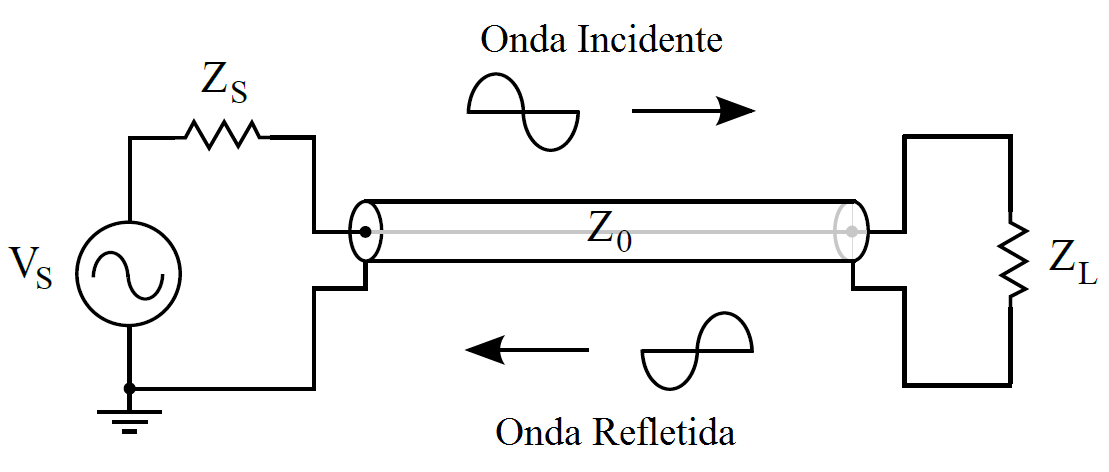
\includegraphics[scale=.4]{./cap2/figuras/incident_reflected.png}
		\caption{Onda incidente e onda refletida em uma linha de transmissão}
		\label{fig:inc_ref}
	\end{center}
\end{figure}

Quando um sinal que está sendo enviado por uma linha de transmissão encontra algum tipo de descontinuidades este então é refletido e segue no sentido oposto ao sinal incidente, como é mostrado na figura \ref{fig:inc_ref}. A velocidade de propagação em uma linha de transmissão pode ser calculada através da equação \ref{eq:velocidade_propagacao}

\begin{equation}
	v_p = \frac{C}{\sqrt{\epsilon_r \mu_r}}
	\label{eq:velocidade_propagacao}
\end{equation}
\noindent
onde \emph{C} é a velocidade de propagação da lu no vácuo, aproximadamente $3.10^8$m/s, $\epsilon_r$ é permissividade relativa do material dielétrico e $\mu_r$ é a permeabilidade relativa do material.

\section{Sistema de Medição}
O sistema para a realização de medições de TDR, é um set-up simples que consiste em um gerador de sinal, que pode ser um degrau ou um impulso, um osciloscópio, que será usado para realizar a leitura do sinal de saída, e o dispositivo a ser medido. O esquemático do sistema de medição é mostrado na figura \ref{fig:circuito_TDR}, onde o sinal do gerador é enviado para o dispositivo em teste através de uma linha de transmissão que possui uma impedância característica $Z_0$, onde convencionalmente o valor assumido dessa impedância é de 50$\Omega$), o sinal após entrar no dispositivo sofre reflexões referentes as descontinuidades e das variações de resistência do dispositivo, este sinal refletido junto com o sinal incidente são então medidos/amostrados pelo osciloscópio pra posteriormente poderem ser analisados

\begin{figure}[htb!]
	\begin{center}
		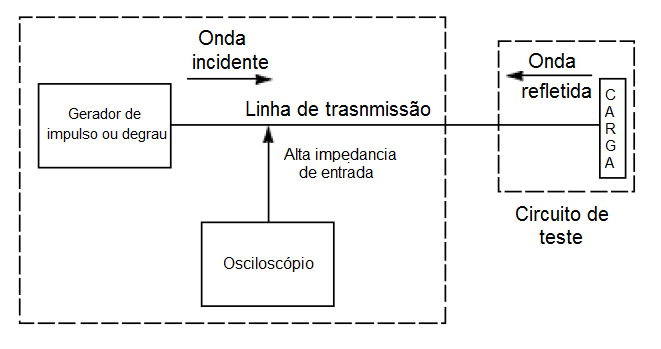
\includegraphics[scale=.6]{./cap2/figuras/simple_TDR.png}
		\caption{Esquema básico para medição TDR}
		\label{fig:circuito_TDR}
	\end{center}
\end{figure}

\section{Sinais de Entrada}

Dois tipos de sinais podem ser utilizados: pulso ou degrau, ambos agem da mesma forma nas medidas, porém, dependo da aplicação em questão uma possui vantagens em relação a outra. A figura \ref{fig:respostas} mostra a resposta para os dois tipos de sinais. O pulso possibilita uma rápida e fácil localização das falhas ou descontinuidades existentes nos sistemas medidos. O degrau também permite uma rápida e fácil localização de falas e descontinuidades, porém, com a vantagem de se obter de forma fácil a impedância no material. Para a pesquisa foi utilizado o degrau que é o sinal utilizado pelo equipamento usado nas medições.

\begin{figure}[htb!]
	\begin{center}
		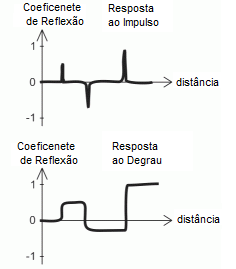
\includegraphics[scale=.9]{./cap2/figuras/tdr_response.png}
		\caption{Respostas típicas para sinais de Pulso e Degrau }
		\label{fig:respostas}
	\end{center}
\end{figure}

Algumas respostas mostradas por esse tipo de medição já são bem conhecidas e equacionadas, entre elas estão a identificação de diferentes impedâncias e os efeitos capacitivos e indutivos que pode aparece ao longo do caminho. Outra resposta é a identificação do final do sistema medido, que pode estar em curto, em aberto ou com alguma carga acoplada nele. 

\section{Amplitude do Sinal Medido}

Para um melhor entendimento será proposto uma modelo simples de medição, onde o que está sendo medido compõe-se de uma linha de transmissão (cabo) e uma carga acoplada ao final, como mostrada na figura \ref{fig:circuito_simples}. A resposta apresentado pelo TDR é uma relação entre a impedância da linha de transmissão e da carga acoplada.

\begin{figure}[htb!]
	\begin{center}
		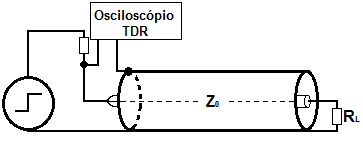
\includegraphics[scale=.7]{./cap2/figuras/simple_circuit_TDR.png}
		\caption{Exemplo de circuito de medição.}
		\label{fig:circuito_simples}
	\end{center}	
\end{figure}

Existem basicamente três casos que podem acontecer: circuito aberto, curto circuito e circuito fechado com carga acoplada; os resultados para cada caso são mostrados na figura \ref{fig:resp_imp}. No caso de circuito aberto a impedância é máxima e o valor mostrado na resposta é a tensão total do pulso incidente. Para para o curto circuito a impedância é mínima logo ocorre o efeito contrario a do circuito aberto, o sinal medido possui valor igual a zero. Já a situação em que há uma carga acoplada no final, podem ocorrer três situações, a primeira é o valor da caga ser igual ao valor da linha de transmissão, assim não havendo mudança no valor medido; a segunda seria com a carga tendo um valor maior que o da linha de transmissão, fazendo com que a diferença entre a relação entre carga e cabo seja positiva; e a terceira e última situação é quando a carga possui valor menor que o cabo, fazendo com que a diferença seja negativa.



\begin{figure}[htb!]
	\begin{center}
		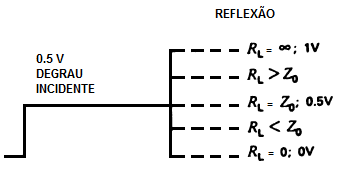
\includegraphics[scale=.7]{./cap2/figuras/resp_impe.png}
		\caption{Resposta para o circuito da figura \ref{fig:circuito_simples}.}
		\label{fig:resp_imp}
	\end{center}	
\end{figure}



\section{Impedância}

Em todo sistema de transmissão um fator físico que sempre deve se levando em consideração é a impedância do sistema. Como já dito o TDR trabalha de forma similar ao radar, onde para cada descontinuidade há uma resposta, mas também mostra a impedância do sistema que é calculado através a amplitude da onda medida. Primeiramente é necessário calcular o coeficiente de reflexão, como mostrado na equação \ref{eq:coe_ref},

\begin{equation}
\rho = \frac{E_r}{E_i} = \frac{R - Z_0}{R + Z_0}
\label{eq:coe_ref}
\end{equation}

Onde $E_r$ é o valor do pulso refletido, $E_i$ é o valor do pulso incidente, $R$ é o valor da carga e $Z_0$ é o valor da impedância da linha de transmissão. Com o valor do coeficiente de reflexão, pode-se deduzir se sistema medido está em curto, aberto ou com alguma carga acoplada. Para isso temos que saber que a quando o valor de $\rho$ = +1 o circuito está aberto, quando $\rho$ = -1, o circuito está em curto, quando $\rho$ = 0 a carga acoplada possui o mesmo valor de impedância que a linha de transmissão, quando 0 < $\rho$ < 1 a carga possui valor maior que a linha de transmissão e quando  -1 < $\rho$ < 0 a carga possui um valor menor, como mostrado na figura \ref{fig:valor_rho}.

\begin{figure}[htb!]
	\begin{center}
		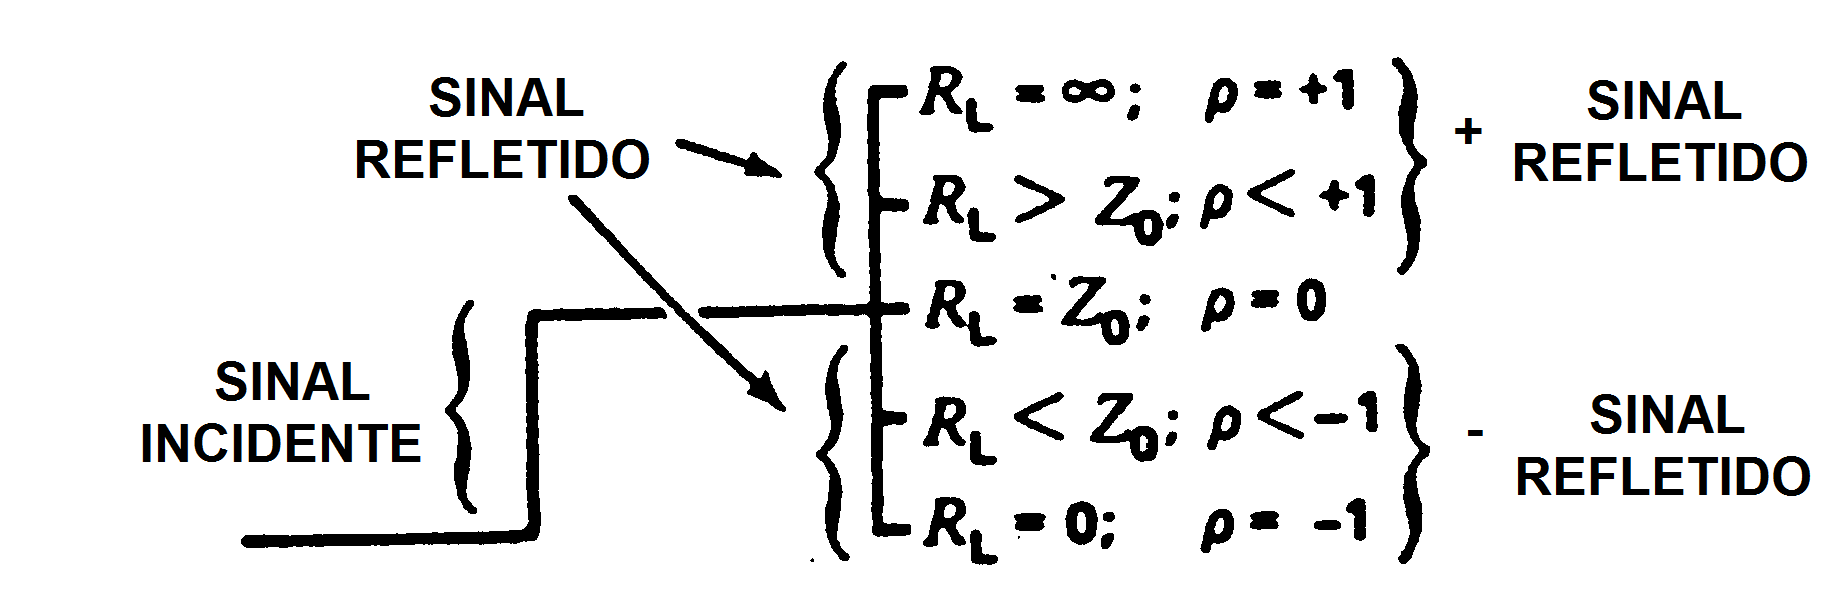
\includegraphics[scale=.18]{./cap2/figuras/tdr_response_reflexao.png}
		\caption{fig:Valores de $\rho$}
		\label{fig:valor_rho}
	\end{center}
\end{figure}

\section{Reflexões Através de Descontinuidades Resistivas}

Dois tipos de reflexões podem ocorrer para dois tipos de descontinuidades resistivas. Eles são uma mudança da reflexão em forma de degrau e uma uma mudança continua da reflexão. Uma resistência em série com uma linha de transmissão causa uma reflexão positiva. A resistência em série com a linha de transmissão causa uma reflexão negativa. Resistores discretos simples causam uma reflexão em degrau, enquanto que resistências distribuídas causa uma mudança contínua. A reflexão para resistores discretos são mostrados de forma ideal na figura \ref{fig:descontinuidade_resistor_simples} e a reflexão para resistência distribuída é mostrada de forma ideal na figura \ref{fig:descontinuidade_resistor_distribuido}.

\begin{figure}[htb!]
	\begin{center}
		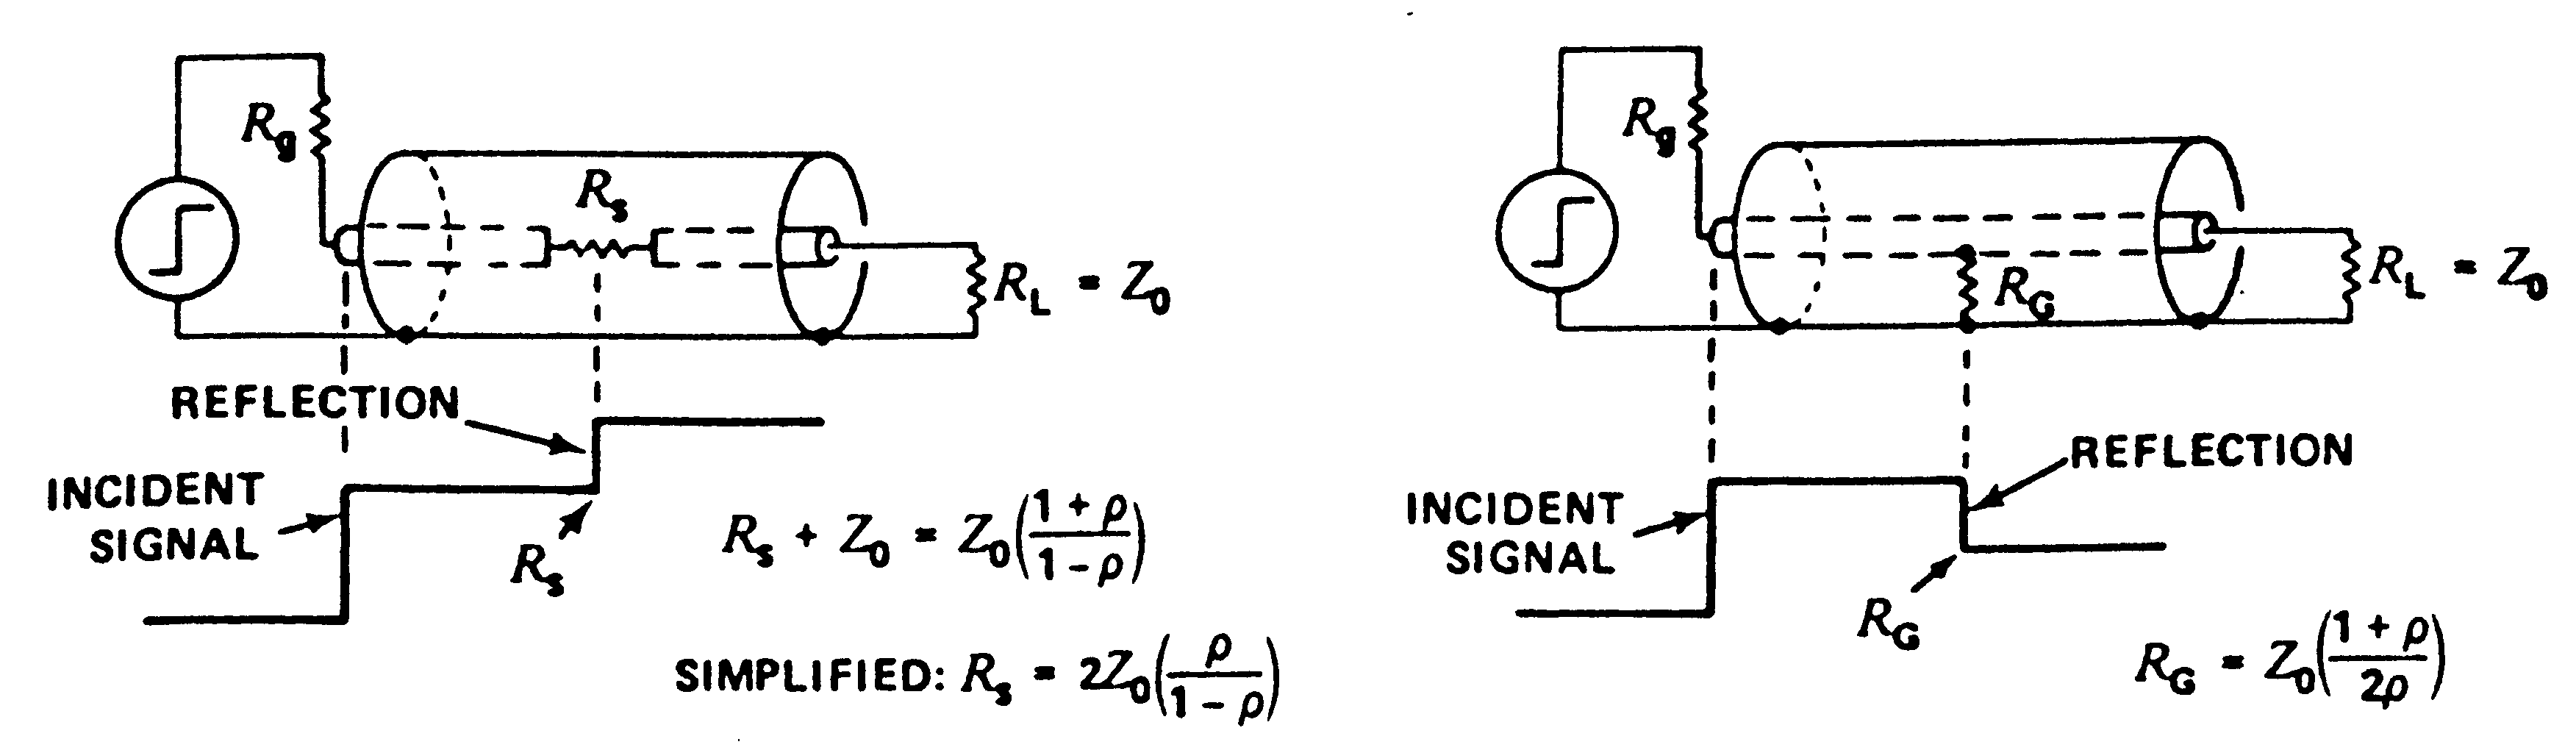
\includegraphics[scale=.15]{./cap2/figuras/discontinuidade_resistor_simples.png}
		\caption{Descontinuidades de Resistores simples e suas reflexões}
		\label{fig:descontinuidade_resistor_simples}
	\end{center}
\end{figure}

\begin{figure}[htb!]
	\begin{center}
		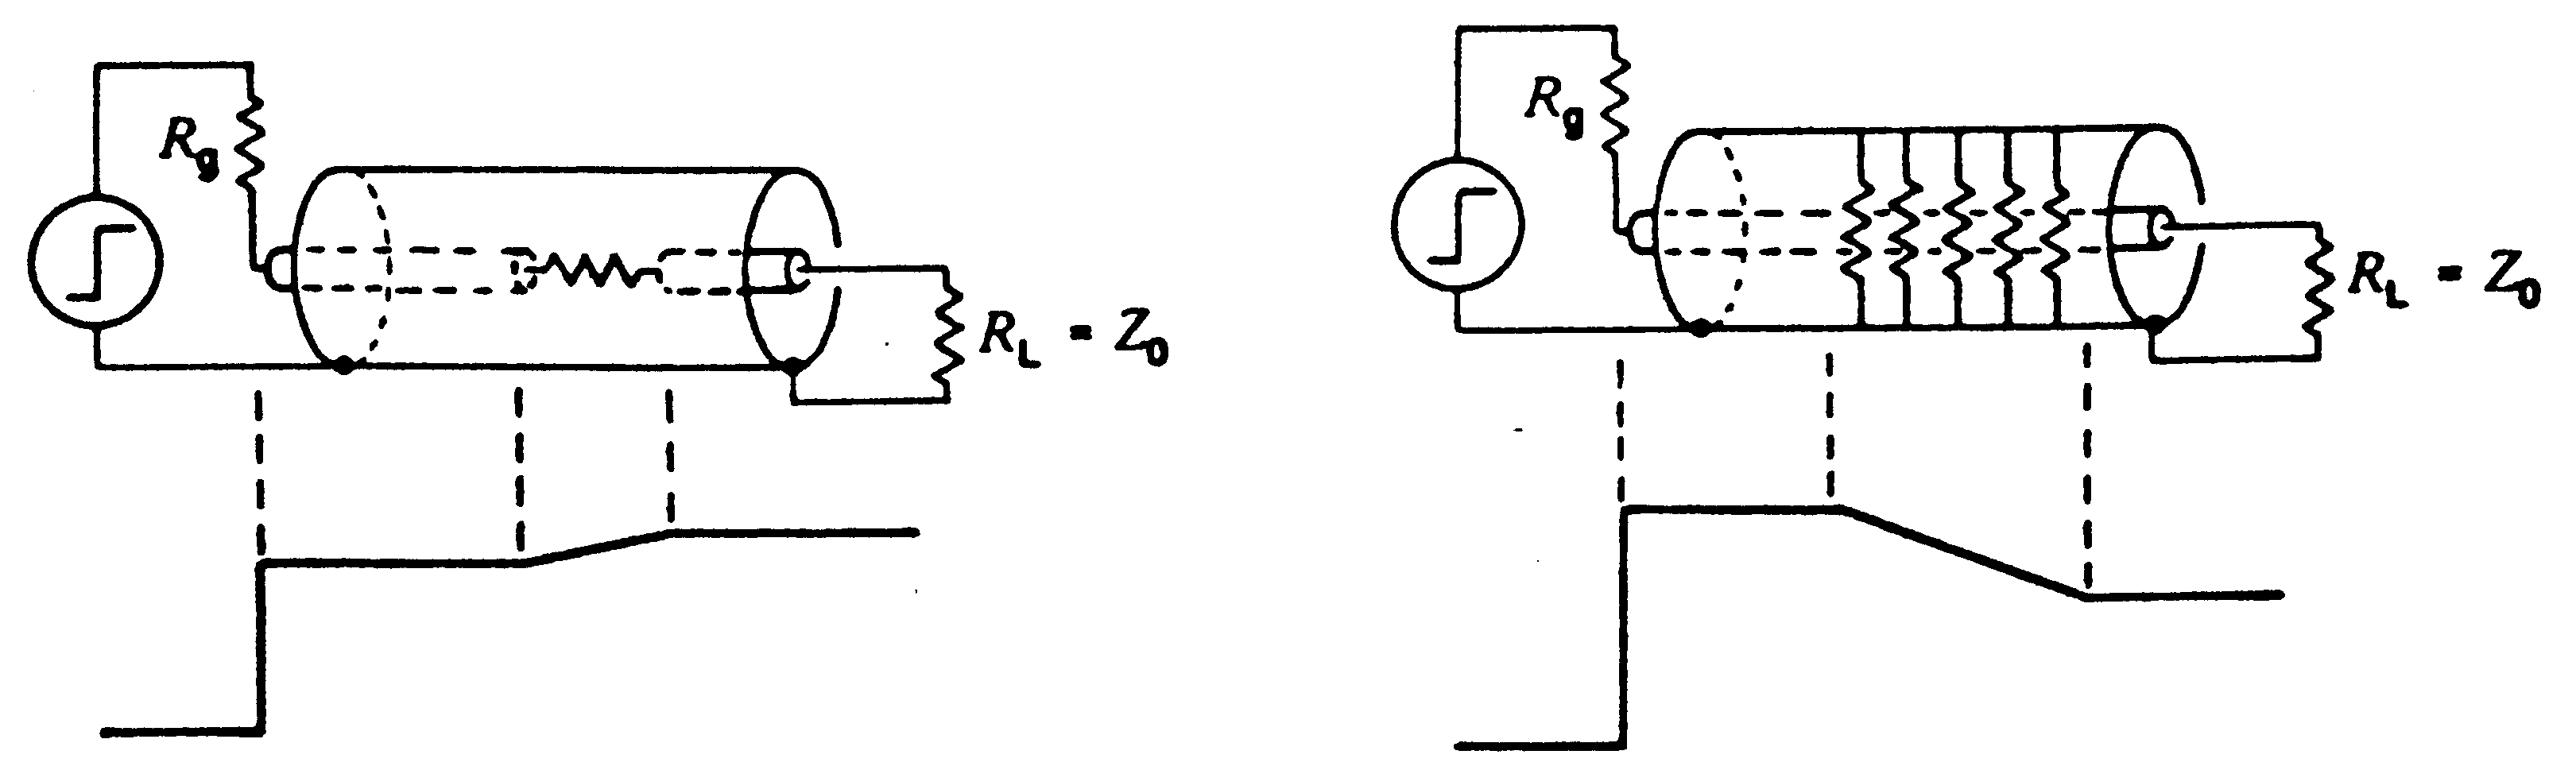
\includegraphics[scale=.15]{./cap2/figuras/discontinuidade_resistor_distrubuido.png}
		\caption{Descontinuidade de resistência distribuída e suas reflexões}
		\label{fig:descontinuidade_resistor_distribuido}
	\end{center}
\end{figure}

A figura \ref{fig:descontinuidade_resistor_distribuido} mostra de forma me exagerada o começo da resistência distribuída em um ponto particular da linha. Normalmente, tando resistência em série quanto em paralelo são encontradas ao longo de toda a extensão de qualquer cabo coaxial testado.

As quatro formas de são uma indicação de perda de sinal entre a entrada e a saída de uma linha de transmissão. A descontinuidade de uma resistor simples pode ocorrer para componentes discretos como um conector solto com adição de uma resistência em série. Tais descontinuidades podem ser localizados fisicamente pelo TDR. Perdas distribuídas são usualmente partes particulares de uma linha que está sendo testada e o display do TDR pode mostrar um valor para uma análise quantitativa de resistência por unidade de tamanho. [\cite{TDK}]
\section{Cargas Capacitivas e Indutivas}

Ao final do sistema medido também podem ser encontradas cargas que nãos seja apenas da resistivas, mas também capacitivas ou indutivas que podem ser encontradas em 2 configurações cada, em série ou em paralelo. Os elementos capacitivos e indutivos possuem comportamentos bem definidos, a seguir são mostrados as respostas para capacitores acoplados.

\begin{figure}[htb!]
	\begin{center}
		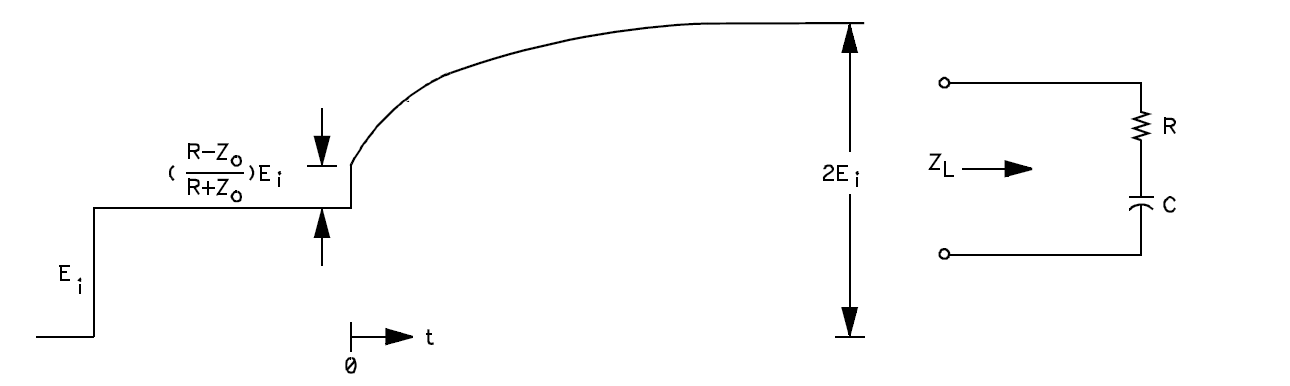
\includegraphics[scale=.30]{./cap2/figuras/R-C_serie_response.png}
		\caption{Circuito R-C em serie}
		\label{fig:RC_serie}
	\end{center}
\end{figure}

\begin{figure}[htb!]
	\begin{center}
		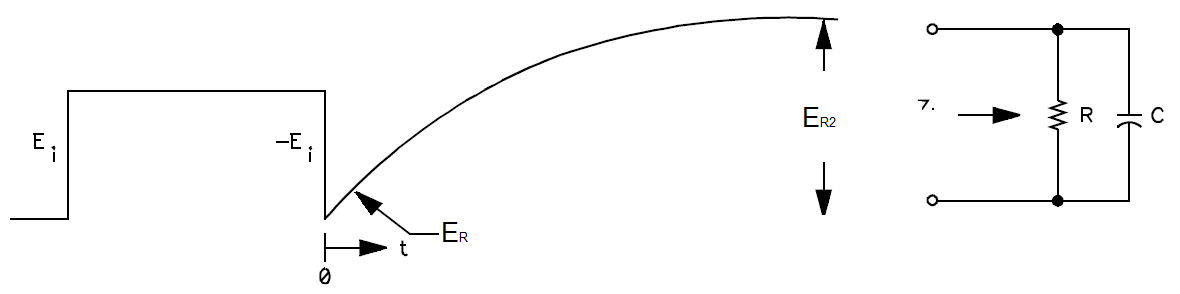
\includegraphics[scale=.30]{./cap2/figuras/R-C_parallel_response.png}
		\caption{Circuito R-C em Paralelo}
		\label{fig:RC_paralelo}
	\end{center}
\end{figure}

Na figura \ref{fig:RC_serie}, a curva de subida do gráfico é pode ser expressa pela equação \ref{eq:RC_serie}.

\begin{equation}
\label{eq:RC_serie}
E_R = E_i\left[(2 - \left(1-\frac{R-z_0}{R+z_0}e^{\frac{-t}{\tau}}\right)\right] \\
\end{equation}

\begin{equation}
\tau = (Z_0+R)C
\end{equation}

E na figura \ref{fig:RC_paralelo}, a curva de subida é dada pelas equações \ref{eq:RC_paralelo} e \ref{eq:RC_paralelo_estacionario}

\begin{equation}
\label{eq:RC_paralelo}
E_R = E_i\left[\left( 1 + \frac{R-Z_0}{R+Z_0}\right)\left( 1 - e^{\frac{-t}{\tau}}\right)\right]
\end{equation}

\begin{equation}
\label{eq:RC_paralelo_estacionario}
E_{R2} = E_i \left(1+ \frac{R-Z_0}{R + Z_0}\right)
\end{equation}

\begin{equation}
\tau = \frac{Z_0R}{Z_0+R}C
\end{equation}

Para a situação da figura \ref{fig:RC_paralelo}, no tempo zero, a carga aparece como um circuito aberto, uma vez que o capacitor não aceita uma repentina repentina de tensão. Portanto $\rho = -1$ quando $t =0$. Após uma espaço de tempo, entretanto, a voltagem em C aumenta e a sua impedância cresce. Em $ t = \inf$, o capacitor torna-se uma circuito aberto. Uma análise semelhante também pode ser feita para a situação apresentada na figura \ref{fig:RC_serie}.[\cite{agilent}]

Para caragas como indutores acopladas ao final do sistemas temos um tipo de resposta diferente que são mostradas nas figuras \ref{fig:RL_serie} e \ref{fig:RL_paralelo}.

\begin{figure}[htb!]
	\begin{center}
		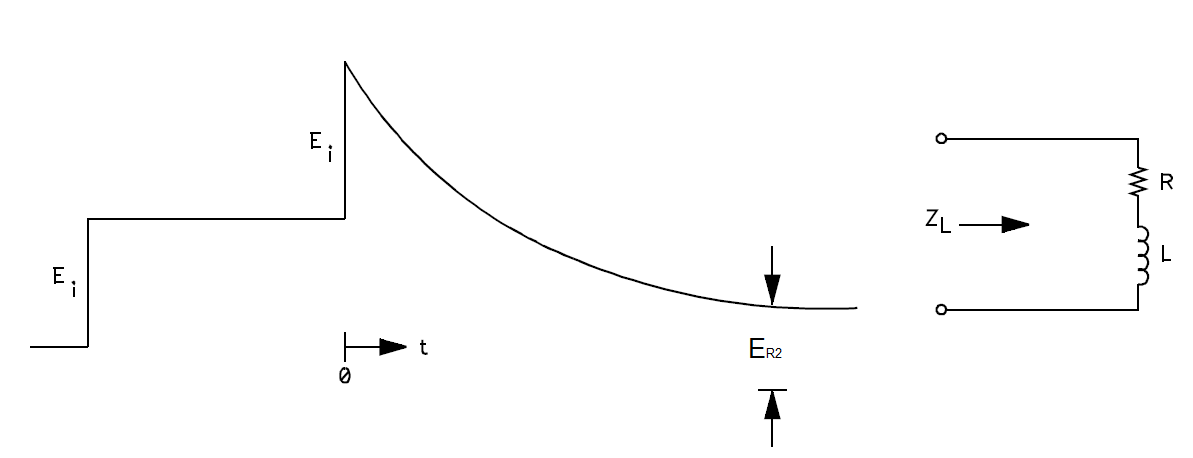
\includegraphics[scale=.30]{./cap2/figuras/R-L_serie_response.png}
		\caption{Circuito R-L em serie}
		\label{fig:RL_serie}
	\end{center}
\end{figure}

\begin{figure}[htb!]
	\begin{center}
		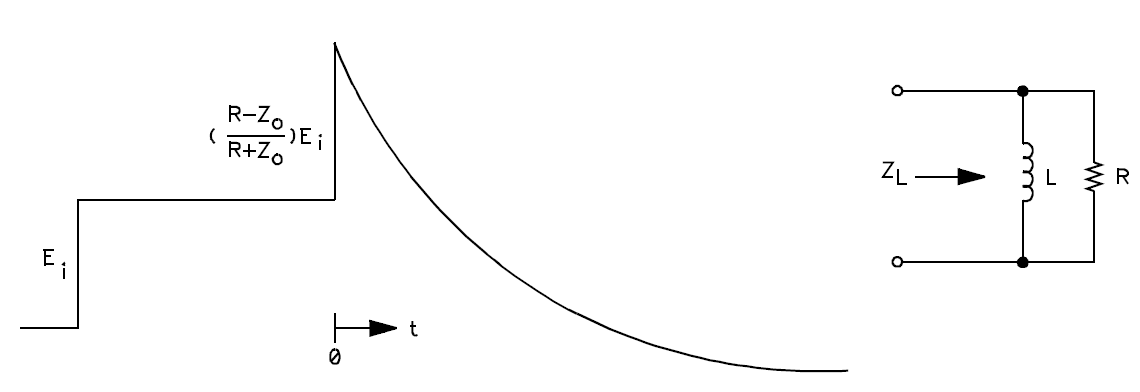
\includegraphics[scale=.30]{./cap2/figuras/R-L_parallel_response.png}
		\caption{Circuito R-L em Paralelo}
		\label{fig:RL_paralelo}
	\end{center}
\end{figure}

A curva de descida mostrada na figura \ref{fig:RL_serie} é definida pelas equações \ref{eq:RL_serie} e \ref{eq:RL_serie_estacionario}.
%
\begin{equation}
\label{eq:RL_serie}
E_R = E_i \left[\left( 1 + \frac{R - Z_0}{R + Z_0}\right) + \left( 1 + \frac{R - Z_0}{R + Z_0}\right) e^{\frac{-t}{\tau}}\right]
\end{equation}

\begin{equation}
\label{eq:RL_serie_estacionario}
E_{R2} =  E_i \left( 1 + \frac{R - Z_0}{R + Z_0}\right) 
\end{equation}

\begin{equation}
\label{eq:tau_RL}
\tau = \frac{L}{R + Z_0}
\end{equation}

E para a situação mostrada na figura \ref{fig:RL_paralelo}, a cura de descida pode ser expressa pela equação \ref{eq:RL_paralelo}.

\begin{equation}
\label{eq:RL_paralelo}
E_R = E_i\left[\left( 1 + \frac{R-Z_0}{R+Z_0}\right)e^{\frac{-t}{\tau}}\right]
\end{equation}


\begin{equation}
\tau = \frac{Z_0+R}{Z_0R}L
\end{equation}

Para o caso mostrado na figura \ref{fig:RL_serie}, no tempo $t = 0$ a tensão refletida é $+E_i$. Isso ocorre porque o indutor não aceita uma mudança repentina na corrente; assim inicialmente comportando-se como uma impedância infinita, e $\rho = +1$ para $t = 0$. Então a corrente aumenta exponencialmente e sua impedância cai para zero. Quando $t \rightarrow \infty$ então $e_r(t)$ é definido somente pelo valor de R. [\cite{agilent}]
O exponencial de transição de $e_r(t)$ tem uma constante de tempo determinada pelar resistência efetiva vista pelo indutor, mostrado na equação \ref{eq:tau_RL}. Uma análise semelhante também pode ser feita para a figura \ref{fig:RL_paralelo}.

Capacitores e indutores também podem aparecer como descontinuidades na linha de transmissão, geralmente elas aparecem em uma forma bem simples, na forma de pequenas ondas, como ilustrado nas figuras \ref{fig:descontinuidade_C_L} e \ref{fig:Descontinuidade_CL}.


\begin{figure}
	\begin{center}
		 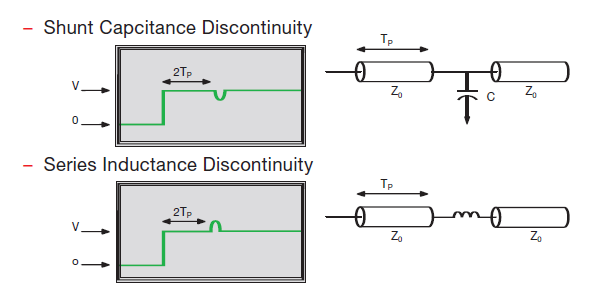
\includegraphics[scale=.5]{./cap2/figuras/C_L_descontinuidade.png}
		 \caption{Descontinuidades capacitivas e descontinuidade indutivas.[\cite{TDK2}]}
		 \label{fig:descontinuidade_C_L}
	\end{center}
\end{figure}


\begin{figure}
	\begin{center}
		 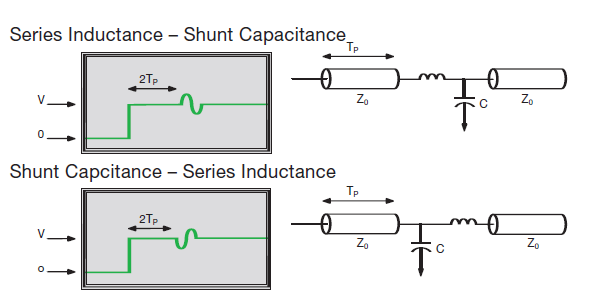
\includegraphics[scale=.5]{./cap2/figuras/CL_descontinuidade.png}
		 \caption{Descontinuidade capacitiva e indutiva. [\cite{TDK2}]}
		 \label{fig:Descontinuidade_CL}
	\end{center}
\end{figure}


\section{Localização de Descontinuidades}

Para a localização da distância da descontinuidade deve-se ter em mão o valor da velocidade de propagação do sinal que é dado por:

\begin{equation}
v_p = \frac{\omega}{\beta} 
\end{equation}
 
ou

\begin{equation}
v_p = \frac{c}{\sqrt{\varepsilon_r}}
\end{equation}

Onde $c$ é a velocidade da luz e $\varepsilon$ é a constante dielétrica do da linha de transmissão. A distancia de propagação é dada por:

\begin{equation}
d = v_pt
\end{equation}

logo 

\begin{equation}
\label{eq:distancia}
d = \frac{c}{\sqrt{\varepsilon_r}}\frac{t_0}{2}
\end{equation}

Onde $t_0$ é a variação do tempo entre o pulso incidente e o pulso refletido. O tempo aparece dividido por dois, pois deve-se levar em consideração que a distancia que o pulso percorre para chegar à descontinuidade e voltar. Dessa forma também podemos calcular a distância entre duas descontinuidades, que é dada por:

\begin{equation}
\Delta d = \frac{c}{\sqrt{\varepsilon_r}}\frac{t_2 - t_1}{2}
\end{equation}

onde $t_1$ é o tempo de viagem nos dois sentidos até a primeira descontinuidade e $t_2$ é o tempo de viagem nos dois sentidos até a segunda descontinuidade. Essas duas descontinuidades podem se tornar indistinguíveis quando separadas por um tempo ($t_2 - t_1$) de metade do tempo de subida do pulso do sistema. Dessa maneira a menor distância para se distinguir duas descontinuidades é dado por 

\begin{equation}
d_{min} = \frac{c}{\sqrt{\varepsilon_r}}\frac{t_r}{4}
\end{equation}

Isso significa que um sistema que possui um tempo de subida de 45ps, duas descontinuidades se juntam e tornam-se indistinguíveis a uma distancia de 3.5mm, utilizando-se o ar como dielétrico. [\cite{agilent}]

\section{Aplicações}

\section{Resumo do Capítulo}

Neste capítulo foi fornecido toda a base teórica necessária para a realização da medição e a análise dos resultado obtidos através do Método de TDR, assim como também mostrar como ele pode ser útil para a aquisição de outros tipos de dados, além apenas da impedância característica do sistema.

